\chapter{Platform as a Service with Openshift}
\label{cha:paas}
Platform as a Service (PaaS) is a cloud service, which provides an on demand platform for building, deploying and running containerized applications in the cloud. PaaS can be seen as an enhancement of CaaS, which has been discussed in Chapter \vref{cha:caas}. A PaaS platform does not only provide a container runtime for running containers in the cloud, but also tooling for building, deploying and monitoring of containerized applications, as well as security mechanisms for securing those applications. There are multiple PaaS providers on the market but the most popular PaaS providers are RedHat Openshift Online, Microsoft Azure Cloud Services, Google App Engine and AWS Elastic Beanstalk. They all bring in their own flavor of PaaS but they all provide similar features expected from a PaaS platform\cite{OpenshiftOnline2018, MicrosoftAzueCloudServices2018, GoogleCloudAE2018, AmazonWebServicesEBT2018}. \\

PaaS providers usually provide templates for the major programming languages, application servers, as well as integrations to other cloud services. External cloud services of the same vendor are usually better supported than cloud services of other vendors. This is normal, because cloud providers want the customers to use their services over the services of the competition. What all PaaS providers have in common, is the consumption based pricing model, whereby only the consumed physical resources have to be paid for, and the ability to scale with the workload. \\ 

IPaaS can be seen as an enhancement of PaaS, which provides special features for implementing an ESB, which is discussed in Chapter \vref{cha:esb}. IPaaS enhances an ordinary PaaS platform by providing tooling for integrating external services effortlessly via a low/no code platform, whereby service integrations can be defined via an UI, rather then by implementing source code. Red Hat Fuse 7 is an example for an IPaaS platform, which will replace JBoss Fuse 6.x in the near future\cite{Fuse72018, iPaaSP12015, iPaaSP22015}. \\

Openshift Origin is an open source PaaS platform, which has been released in April 2012 and is the upstream project for Red Hat Openshift Enterprise. Before Openshift 3 (Jun 2013), Openshift used its own container runtime and orchestration tooling, which since Openshift 3, have been replaced by Docker and Kubernetes, because of its popularity and general availability. Openshift is the only major PaaS platform of the previously noted ones, which can be self hosted or hosted by a local provider. The other major PaaS providers, such as Microsoft Azure, are only available as a cloud service, which are hosted in the vendors data centers\cite{OpenshiftOriginGithub2018}.

\section{The need for Platform as a Service}
\label{sec:paas-need-for-paas}
PaaS platforms like Openshift are based on a CaaS platform, and enhance CaaS by providing a web console, and templates, which allow to define all necessary resources for a service, as well as its release behavior. An instance of a service can be created via the web console, whereby only the required values for the exposed parameters of the template have to be provided. CaaS alone is suitable if its used by developers, but is not suitable for persons without any deep knowledge of containerization and container orchestration. This is where PaaS platforms come into place. Developers specify templates for the provided services, which specify the necessary service resources, and non-developers create a service instance via the web console. The PaaS platform takes the template and provided template parameter values and provisions the service for the user. \\

Enterprises can profit from PaaS platforms, by defining templates for services they provide for their departments, partners or customers, who can create an instance of a service on demand, and destroy it if not needed anymore. PaaS platforms provide a self service console, where services can be created, managed and destroyed effortlessly, without the need to understand the underlying platform. The self service console could be implemented by enterprises for their specific use cases, whereby the custom self service console interacts with PaaS platform via its exposed REST API. \\

PaaS platforms like Openshift usually provide an integration in a Continuous Integration / Continuous Deployment (CI/CD) workflow, which allows to automatically build and deploy new service releases on the PaaS platform in a predefined manner. Therefore, the PaaS platforms are integrated in the whole software life-cycle. This decreases the effort of the developers to interact with the cloud platform and provides additional automation.
 
\section{Openshift}
\label{sec:paas-openshift}
Openshift is a open source PaaS platform, which uses Docker as the container runtime and Kubernetes for the container orchestration. Openshift is designed as a client server architecture and a master slave architecture, the same way as Kubernetes, which has been discussed in Section \vref{sec:caas-kubernetes}. An Openshift Cluster can contain multiple Kubernetes Clusters, which are managed by the Openshift Master. Openshift introduces the concept of a project, which is actually a Kubernetes Namespace, whereby a project is completely isolated from other projects. Figure \vref{fig:paas-openshift-kubernetes-cluster-architecture} illustrates the architecture of an Openshift Cluster\cite{OpenshiftDeepDive2014, OpenshiftCoreConcepts2018}.

\begin{figure}
	\centering
	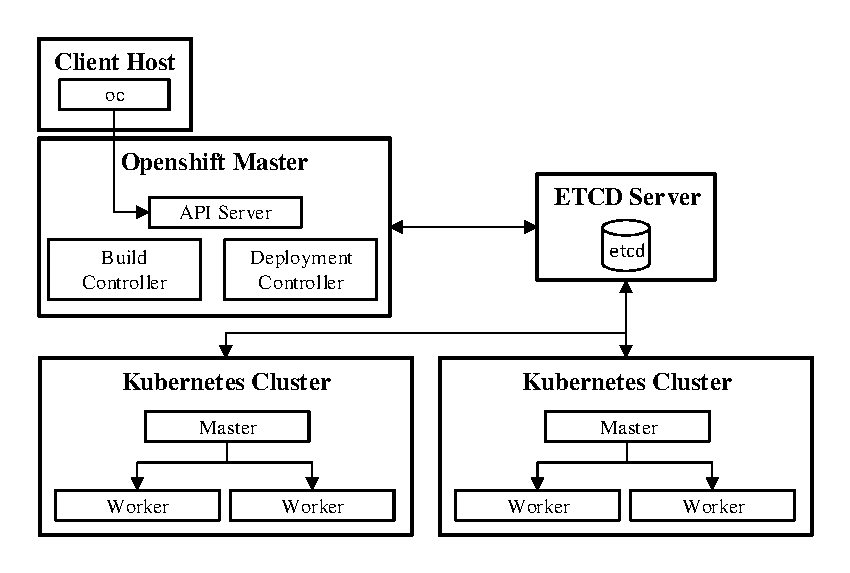
\includegraphics[scale=1]{images/openshift-kubernetes-cluster-architecture.pdf}
	\caption{Architecture of an Openshift Cluster}
	\label{fig:paas-openshift-kubernetes-cluster-architecture}
\end{figure} 

\subsection{Openshift Master}
\label{sec:paas-openshift-master}
The Openshift Maser manages the Kubernetes Master of the Kubernetes Clusters the Openshift Cluster contains. The Openshift Master exposes a REST API via the clients can interact with the Openshift Cluster. Openshift is placed on top of Kubernetes, whereby the Openshift Master node acts similar as a Kubernetes Master node, which has been discussed in Section \vref{sec:caas-kubernetes-master}. Additionally, Openshift provides features, which are not provided by Kubernetes, such as, a role and group based security model for isolating the Kubernetes Namespaces via Openshift Projects, and controllers for managing the additional Openshift Objects. The following Section will discuss the Openshift Project, which is one of the new features provided by Openshift.

\subsection{Openshift Project}
\label{sec:paas-openshift-project}
An Openshift Project represents a Kubernetes Namespace, where all resources of an Openshift Project are located. An Openshift Project provides the isolation and security for a Kubernetes Namespace, which are not provided by Kubernetes itself. Figure \vref{fig:paas-openshift-project-architecture} illustrates the Openshift Project architecture, its contained objects, and their dependencies to each other. The bold marked objects represent the new objects, which were introduced by Openshift.
\newpage

\begin{figure}[htbp]
	\centering
	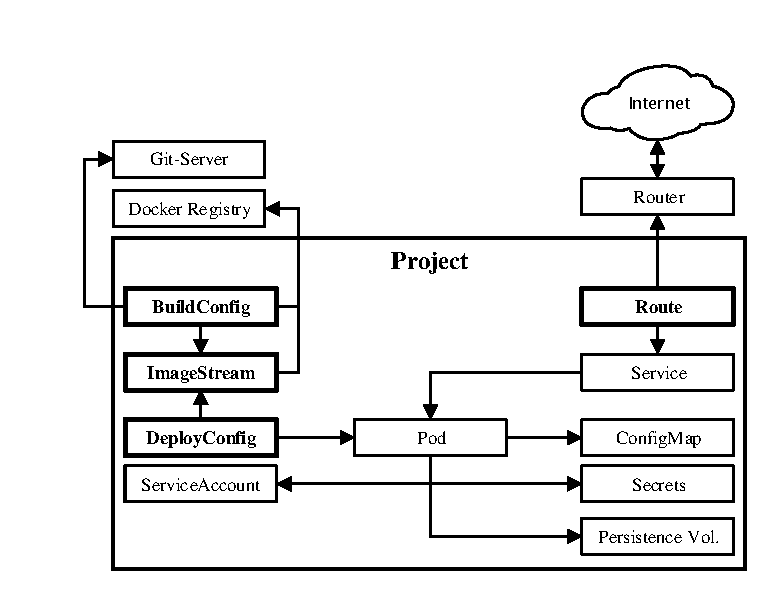
\includegraphics[scale=1]{images/openshift-project-architecture.pdf}
	\caption{Architecture of an Openshift Project}
	\label{fig:paas-openshift-project-architecture}
\end{figure} 

Openshift Objects are persistent objects in the Openshift System, and the Openshift Objects describe the state of the Openshift Cluster. This behavior has been inherited from the underlying Kubernetes System, as discussed in Section \vref{sec:caas-kubernetes-objects}. The following sections briefly introduce the new objects provided by Openshift. 

\mysubsubsection{Openshift BuildConfig}
An Openshift BuildConfig specifies the way how a Docker Image is built on the Openshift Cluster, whereby the built Docker Image is pushed into the Openshift internal Docker Registry. An Openshift BuildConfig supports the following listed strategies:
\begin{itemize}
	\item The \emph{Source-to-Image (S2I)} strategy, is the build strategy, which builds a Docker Image from application source code with a so called builder image.
	\item The \emph{Docker} strategy, is the build strategy, which builds a Docker Image from a Dockerfile.
	\item The \emph{Custom} strategy, is the build strategy, which builds a Docker Image with a custom implemented build mechanism.
	\item The \emph{Pipeline} strategy, is the build strategy, which performs a Jenkins Pipeline build on a Jenkins build server.
\end{itemize}

The sources for a build are provided via a git repository, and an Openshift BuildConfig can be triggered via a web hook by an external git server\cite{S2I2018, OpenshiftBuildStrategies2018}. 

\mysubsubsection{Openshift ImageStream}
An Openshift Image Stream and its Image Stream-Tags are an abstraction of the actual used Docker Image, and an Image Stream uses the same naming convention as Docker Tags (E.g \mentionedtext{myproject/app:1.0}), whereby
\begin{itemize}
	\item \mentionedtext{myproject} represents the Image Stream namespace,
	\item \mentionedtext{app} represents the Image Stream and
	\item \mentionedtext{1.0} represents the Image Stream-Tag.
\end{itemize}
An Image Stream-Tag references a Docker Image instance by its Docker Image-Id, because a Docker Image-Id always references the same Docker Image instance, whereby a Docker Image-Tag can reference different Docker Image instances. Once the Docker Image has been imported, it will not be automatically pulled again, unless the Image Stream-Tag is named \mentionedtext{latest}. \\

A Docker Image can be updated in a Docker Registry, which would break the consistency principle, because it wouldn't be the same Docker Image as used before the update. An Image Stream, in particular the Image Stream-Tag, avoids this by referencing the Docker Image-Id, which makes a used Docker Image immutable within an Openshift Project, unless the name \mentionedtext{latest} is used for the Image Stream-Tag\cite{OpenshiftBuildAndImageStreams2018}.

\mysubsubsection{Openshift DeployConfig}
An Openshift DeployConfig specifies how a deployment of a Pod has to be performed. An Openshift DeployConfig allows to specify the Kubernetes life-cycle hooks pre-hook or post-hook, which are used to configure the deployed Pod before its process has started (pre-hook) or after its process has started and is ready (post-hook). An Openshift DeployConfig supports the following listed deployment strategies\cite{OpenshiftDeployments2018}:
\begin{itemize}
	\item The \emph{Rolling} strategy, is the deployment strategy, which waits for the new deployment to be ready before the old deployment gets removed.
	\item The \emph{Recreate} strategy, is the deployment strategy, which removes the old deployment when the new deployment gets started.
	\item The \emph{Custom} strategy, is the deployment strategy, which performs the deployment by a custom implementation.
\end{itemize}

\mysubsubsection{Route}
An Openshift Route exposes a Service with a host name to an external network, so that it can be reached by its host name from outside the Openshift Project. The Route is deployed on an Openshift Router, which performs the routing between the external network and the connected Openshift Service. A Route can be secured with TLS, whereby the certificates of the Openshift Cluster can be used, or the certificate can be directly defined on the Openshift Route. \\

The following section will discuss the Enterprise Service Bus, which will be implemented by the prototype and hosted on an Openshift Cluster.